\section{Centered-square results}
\label{app:square}


This appendix provides the complete centered-square overlap results
underlying the main-text routing and fusion comparison. Table~\ref{tab:square_fusion_full} reports the velocity, pressure,
and joint errors for the individual specialists and the fusion baselines in the $S$--$H$ and $H$--$P$ overlap regions. In the main text, ``Best fixed'' denotes the fixed specialist with the
lowest aggregate joint error over the corresponding overlap, whereas the convex oracle is a window-wise a posteriori reference.



\paragraph{Overlap evaluation and descriptor ablation.}
For both overlaps, $E_u$, $E_p$, and $E_{\mathrm{joint}}=E_u+E_p$ are reported at the terminal rollout step ($k=24$) and averaged over 16 held-out windows.  This terminal metric differs from the full-window objective used by the diagnostic convex oracle. To assess the role of history information in the second routing level, we also include T2-C $\mu$-only, which uses the same correction-gate architecture and training protocol as T2-C but removes the standardized history descriptor by setting its channels to zero. Table~\ref{tab:square_fusion_full} reports the validation-selected comparison, and the corresponding three-seed gate variability is summarized separately below.

\par
\begin{table}[H]
\centering
\caption{
Centered-square routing and fusion errors at $K=24$. The convex oracle is an a posteriori reference unavailable during prediction.
T2-C $\mu$-only uses the same gate architecture as T2-C but removes the standardized history descriptor. Bold indicates the best deployable method within each overlap.
}
\label{tab:square_fusion_full}
\small
\setlength{\tabcolsep}{5pt}
\begin{tabular}{@{}llrrr@{}}
\toprule
Overlap & Predictor & $E_u$ & $E_p$ & $E_{\mathrm{joint}}$ \\
\midrule
$S$--$H$ & Steady specialist & 2.5976 & 2.2450 & 4.8426 \\
 & Hopf specialist & 0.4942 & 1.2356 & 1.7298 \\
 & E2 Top-1 & 0.4942 & 1.2356 & 1.7298 \\
 & Equal blend & 1.3644 & 1.6677 & 3.0321 \\
 & E2-probability blend & 0.7898 & 1.3949 & 2.1847 \\
 & T2-C $\mu$-only & 0.7898 & 1.3948 & 2.1846 \\
 & T2-C & \textbf{0.4615} & \textbf{0.7343} & \textbf{1.1958} \\
 & Convex oracle & 0.4659 & 0.7183 & 1.1842 \\
\midrule
$H$--$P$ & Periodic specialist & 0.6420 & 0.5659 & 1.2079 \\
 & Hopf specialist & 1.0034 & 1.8684 & 2.8718 \\
 & E2 Top-1 & 0.7422 & 1.1052 & 1.8473 \\
 & Equal blend & 0.6077 & 1.0069 & 1.6146 \\
 & E2-probability blend & 0.6154 & 1.0464 & 1.6618 \\
 & T2-C $\mu$-only & 0.5875 & 0.5629 & 1.1504 \\
 & T2-C & \textbf{0.4509} & \textbf{0.3956} & \textbf{0.8465} \\
 & Convex oracle & 0.4479 & 0.3905 & 0.8384 \\
\bottomrule
\end{tabular}
\end{table}
\par

\par
\begin{table}[H]
\centering
\caption{
Parameter-wise centered-square routing and T2-C results at $K=24$.
Joint errors and relative reductions are reported in percent.
The mean weight is the Steady-specialist weight for $S$--$H$
and the Periodic-specialist weight for $H$--$P$.
}
\label{tab:square_parameter}
\small
\setlength{\tabcolsep}{3.5pt}
\begin{tabular}{lrlrrrr}
\toprule
Overlap & $Re$ & E2 choice & $\bar\alpha$ & E2 $E_{\mathrm{joint}}$ & T2-C $E_{\mathrm{joint}}$ & Reduction \\
\midrule
$S$--$H$ & 95.1 & Hopf & 0.0967 & 1.7140 & 1.1827 & 31.00\% \\
$S$--$H$ & 95.3 & Hopf & 0.0971 & 1.7456 & 1.2090 & 30.74\% \\
$H$--$P$ & 100.5 & Hopf & 0.5870 & 2.6485 & 0.8571 & 67.64\% \\
$H$--$P$ & 102.0 & Periodic & 0.7094 & 1.0462 & 0.8360 & 20.09\% \\
\bottomrule
\end{tabular}
\end{table}
\par

The regime-local specialists also exhibit low aggregate physical-field errors under their respective held-out evaluations: $(E_u,E_p)=(1.5311,1.4583)\%$ in the Steady regime, $(0.4387,0.4844)\%$ in the Hopf regime, and $(0.9395,1.0921)\%$ in the Periodic regime. Within the overlap evaluations, however, the more accurate individual specialist differs by interface: the Hopf specialist is the better single-model reference in $S$--$H$, whereas the Periodic specialist is more accurate in $H$--$P$. This overlap dependence motivates an adaptive assembly rule rather than a fixed specialist choice across neighboring regimes.





\paragraph{Gate-training seed variability.}
To assess the sensitivity of the second routing level, we retrain only the
T2-C gate for seeds 42001, 42002, and 42003, keeping the specialists, E2
router, candidate rollouts, data splits, and normalization fixed. Full T2-C
and the architecture-matched $\mu$-only variant share the optimization and
selection protocol in Appendix~\ref{app:implementation}.
Table~\ref{tab:t2c_seed_variability} reports the mean and sample standard
deviation ($N=3$, denominator $N-1$), and Table~\ref{tab:t2c_seedwise}
lists the seed-wise joint errors. These statistics describe gate-training
variability, not across-$Re$ variation, a confidence interval, or
full-pipeline uncertainty.

\par
\begin{table}[H]
\centering
\caption{
Three-seed variability of the centered-square T2-C gate at the $K=24$
terminal step. Values are reported as mean $\pm$ sample standard deviation across gate-training seeds.
}
\label{tab:t2c_seed_variability}
\small
\setlength{\tabcolsep}{4pt}
\begin{tabular}{@{}llccc@{}}
\toprule
Overlap & Gate & $E_u$ & $E_p$ & $E_{\mathrm{joint}}$ \\
\midrule
$S$--$H$ & T2-C $\mu$-only & $0.79006\pm0.00026$ & $1.39498\pm0.00012$ & $2.18504\pm0.00038$ \\
 & Full T2-C & $\mathbf{0.46156\pm0.00004}$ & $\mathbf{0.73416\pm0.00014}$ & $\mathbf{1.19572\pm0.00010}$ \\
\midrule
$H$--$P$ & T2-C $\mu$-only & $0.59067\pm0.00461$ & $0.56050\pm0.00435$ & $1.15116\pm0.00070$ \\
 & Full T2-C & $\mathbf{0.45211\pm0.00138}$ & $\mathbf{0.39793\pm0.00215}$ & $\mathbf{0.85004\pm0.00347}$ \\
\bottomrule
\end{tabular}
\end{table}
\par

\par
\begin{table}[H]
\centering
\caption{
Seed-wise centered-square terminal joint errors $E_{\mathrm{joint}}$ (\%) at $K=24$.
}
\label{tab:t2c_seedwise}
\small
\begin{tabular}{@{}llrrr@{}}
\toprule
Overlap & Gate & 42001 & 42002 & 42003 \\
\midrule
$S$--$H$ & T2-C $\mu$-only & 2.18460 & 2.18524 & 2.18527 \\
 & Full T2-C & \textbf{1.19584} & \textbf{1.19567} & \textbf{1.19565}\\
\midrule
$H$--$P$ & T2-C $\mu$-only & 1.15037 & 1.15170 & 1.15143 \\
 & Full T2-C & \textbf{0.84653} & \textbf{0.85011} & \textbf{0.85348} \\
\bottomrule
\end{tabular}
\end{table}
\par

Full T2-C improves upon T2-C $\mu$-only for all three paired seeds in both overlaps. The corresponding reductions in mean joint error are $45.28\%$ in $S$--$H$ and $26.16\%$ in $H$--$P$. In the $S$--$H$ overlap, the $\mu$-only gate remains close to the E2-probability blend, whereas in $H$--$P$ it provides a moderate correction.
In both cases, incorporating the history descriptor yields a further and consistent improvement. These results support the use of history-conditioned assembly in the present centered-square setting.


Figures~\ref{fig:app_square_sh_full} and \ref{fig:app_square_hp_full} provide complete views of the velocity, gauge-corrected pressure, and pointwise error. In the S--H overlap, the Steady and Hopf predictions differ mainly in the near-wake recirculation region and in the downstream pressure-recovery pattern. The T2-C reconstruction remains visually close to the more accurate Hopf prediction while reducing localized discrepancies in both velocity and pressure, consistent with the error reductions reported in Tables~\ref{tab:square_fusion_full} and \ref{tab:square_parameter}.

In the H--P overlap, the discrepancy between the Hopf and Periodic specialists is more pronounced around the obstacle corners, the separated shear layers, and the developing wake. The T2-C reconstruction reduces these localized errors while preserving the dominant large-scale wake structure, consistent with the substantially lower joint velocity--pressure errors reported for this overlap.

\par
\begin{figure}[p]
\centering
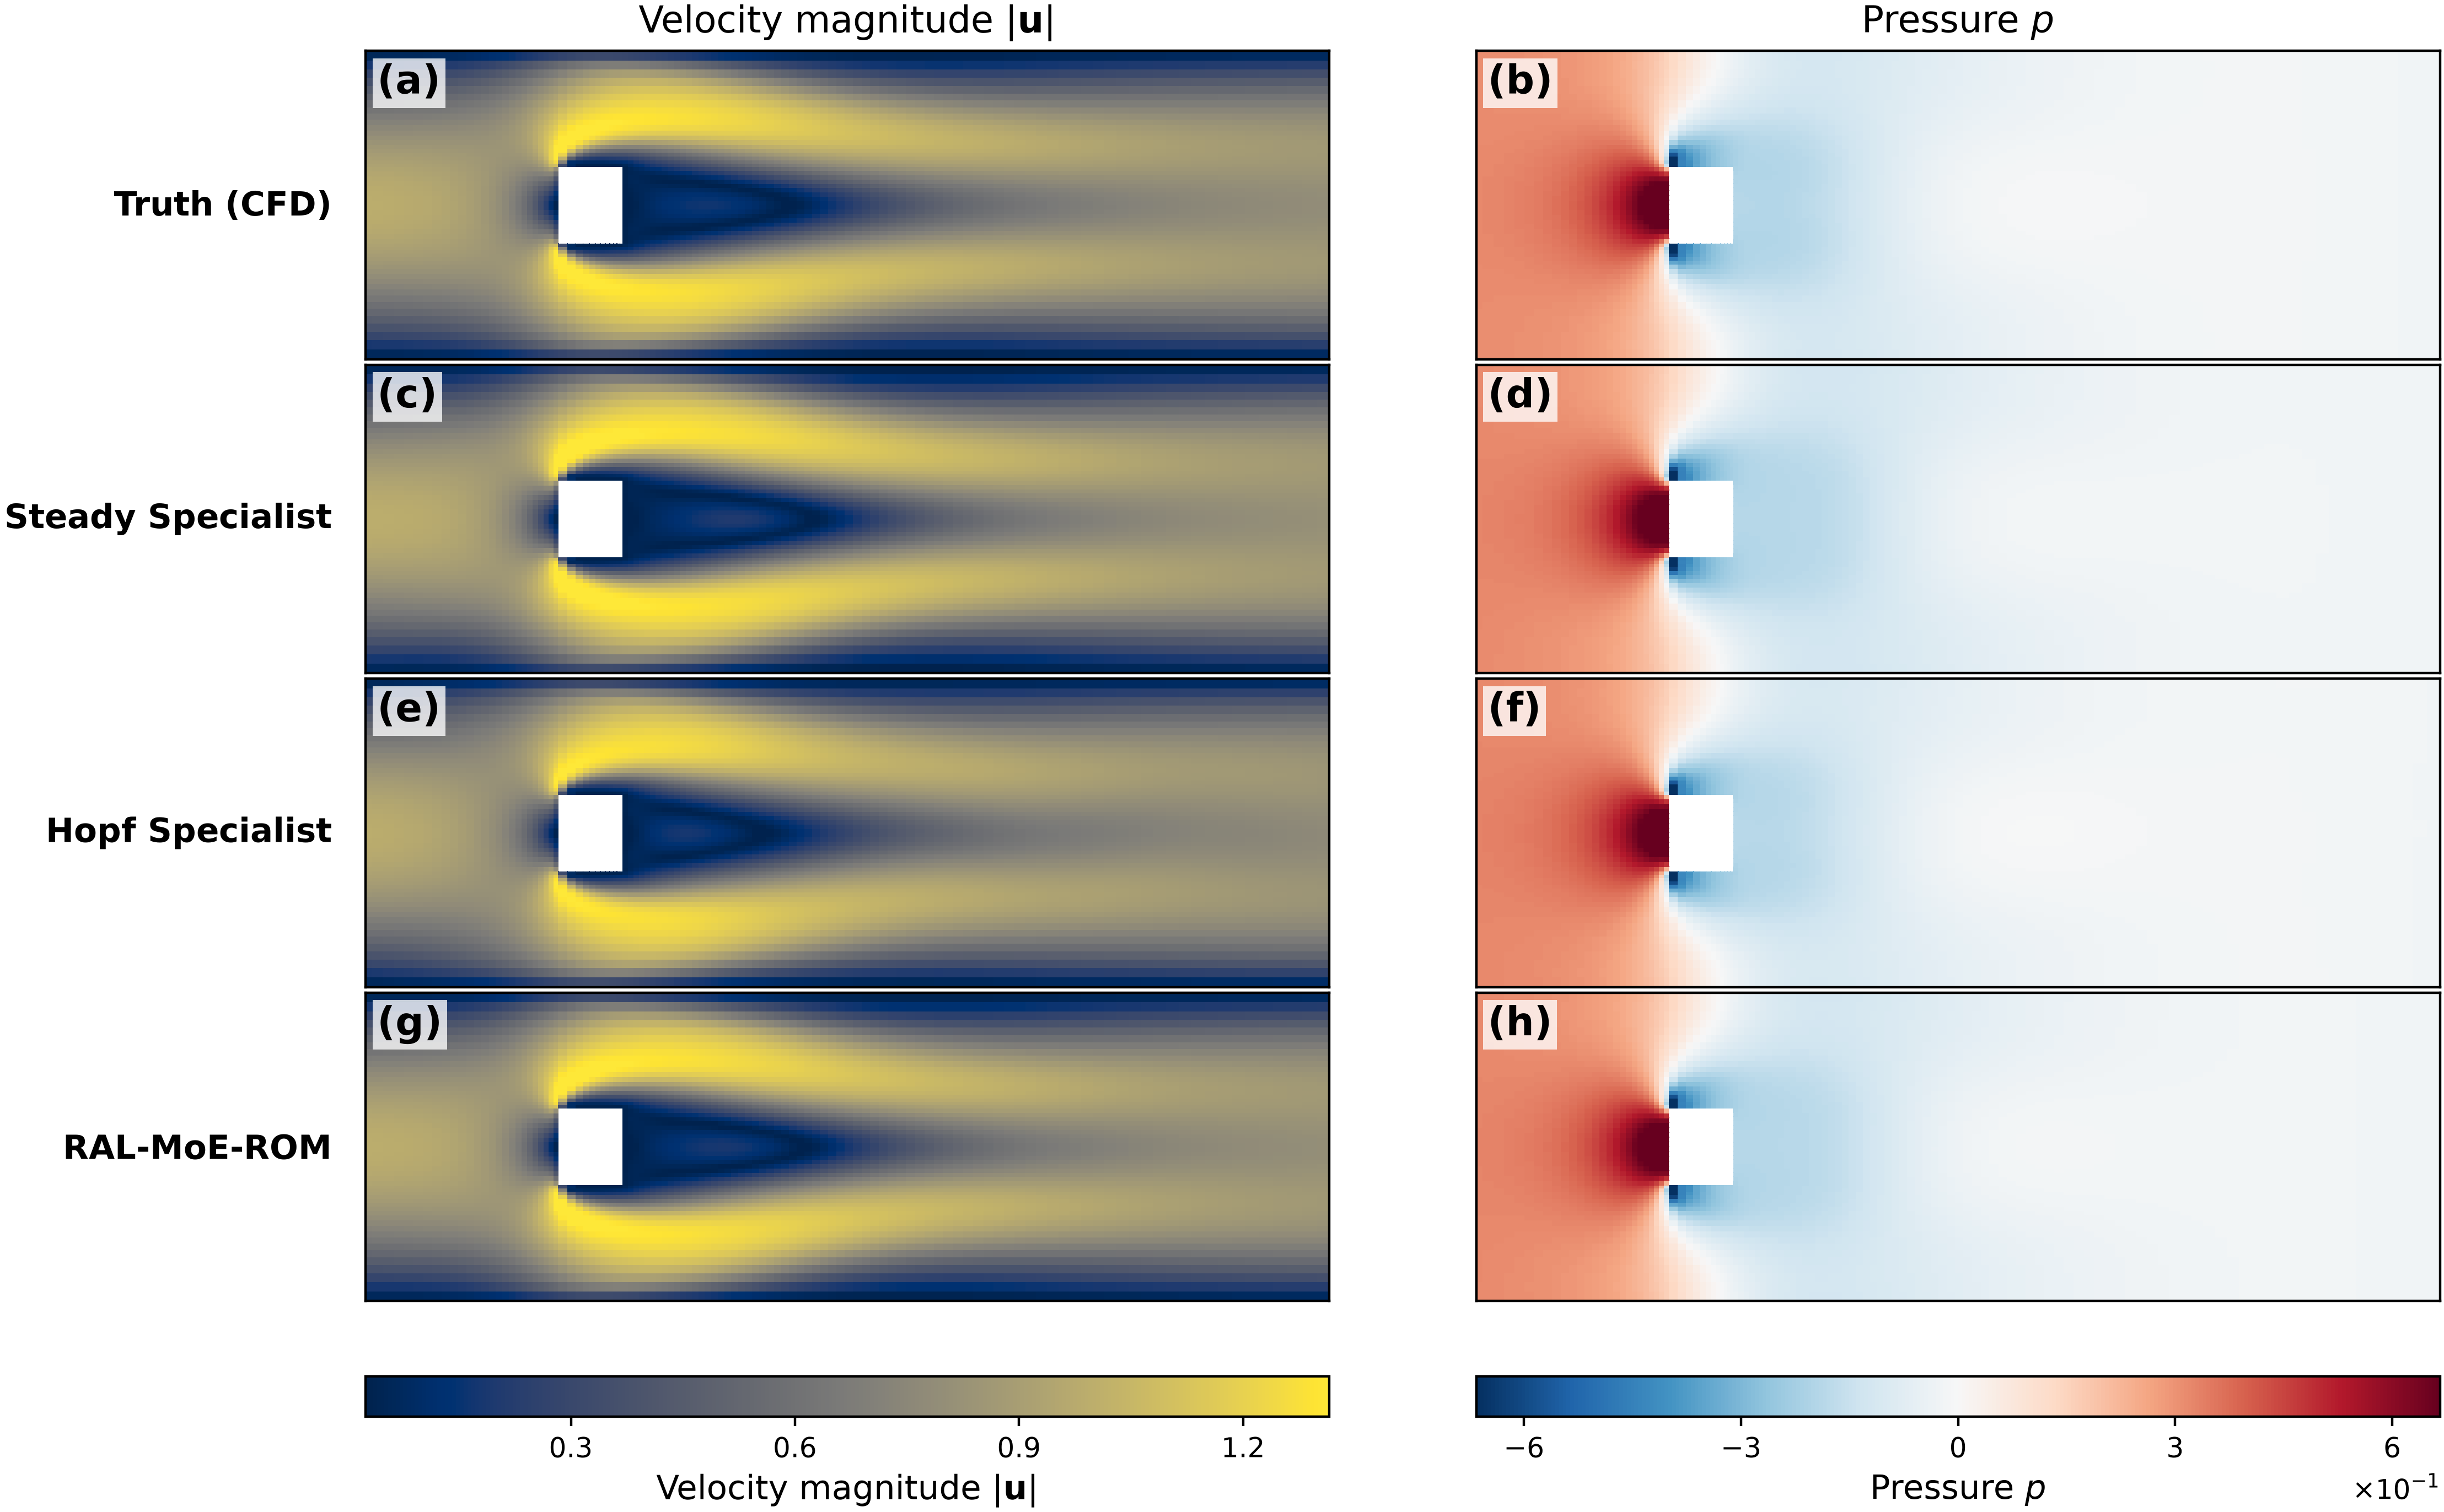
\includegraphics[width=0.95\linewidth]{figures/verified_20260920/SH_fields.png}

\vspace{0.35em}
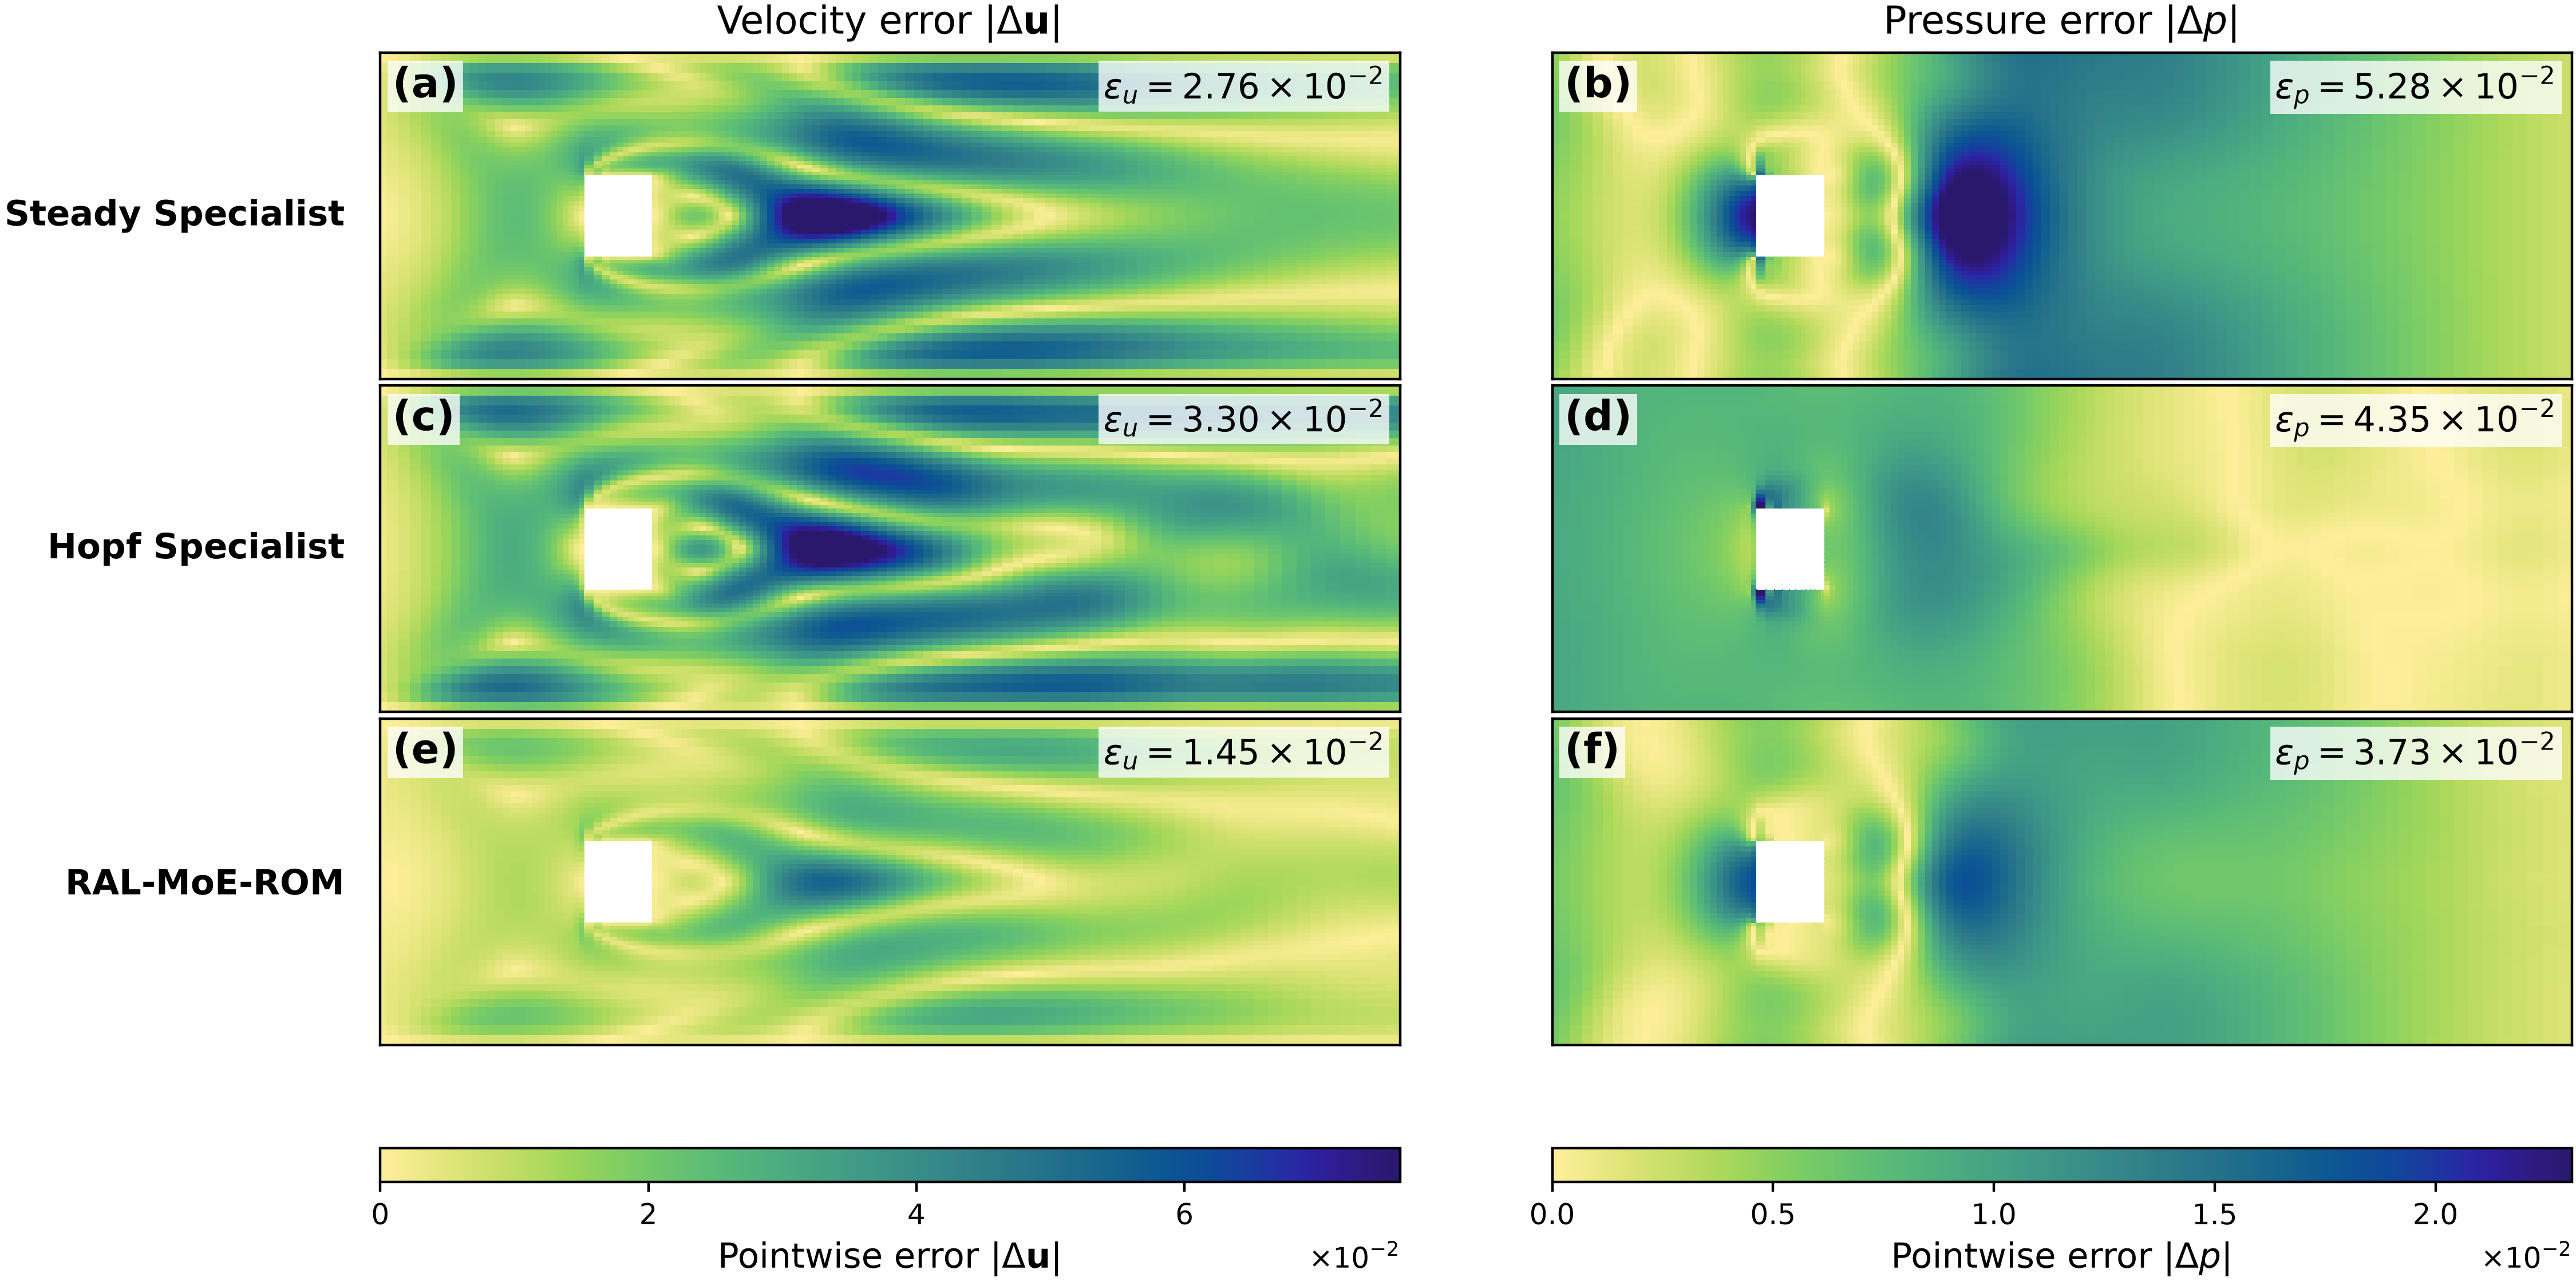
\includegraphics[width=0.95\linewidth]{figures/verified_20260920/SH_errors.png}
\caption{Selected held-out prediction in the centered-square
$S$--$H$ overlap at $Re=95.1$, window 0, zero-based rollout index 1, $t=16$ (not the $K=24$ endpoint). The upper panel compares the CFD reference,
Steady specialist, Hopf specialist, and T2-C prediction for velocity
magnitude and gauge-corrected pressure. The lower panel gives the
corresponding velocity-vector error $\|\widehat{\bm u}-\bm u\|_2$ and absolute pressure error. The archived selection favors fusion advantage and field structure. Shared physical-field scales use CFD-reference quantiles; shared error scales use robust limits over all displayed methods, so extreme values can saturate. Error annotations are relative $L^2$ fractions, not percentages. This is a qualitative example, not an aggregate accuracy estimate.}
\label{fig:app_square_sh_full}
\end{figure}
\par

\par
\begin{figure}[p]
\centering
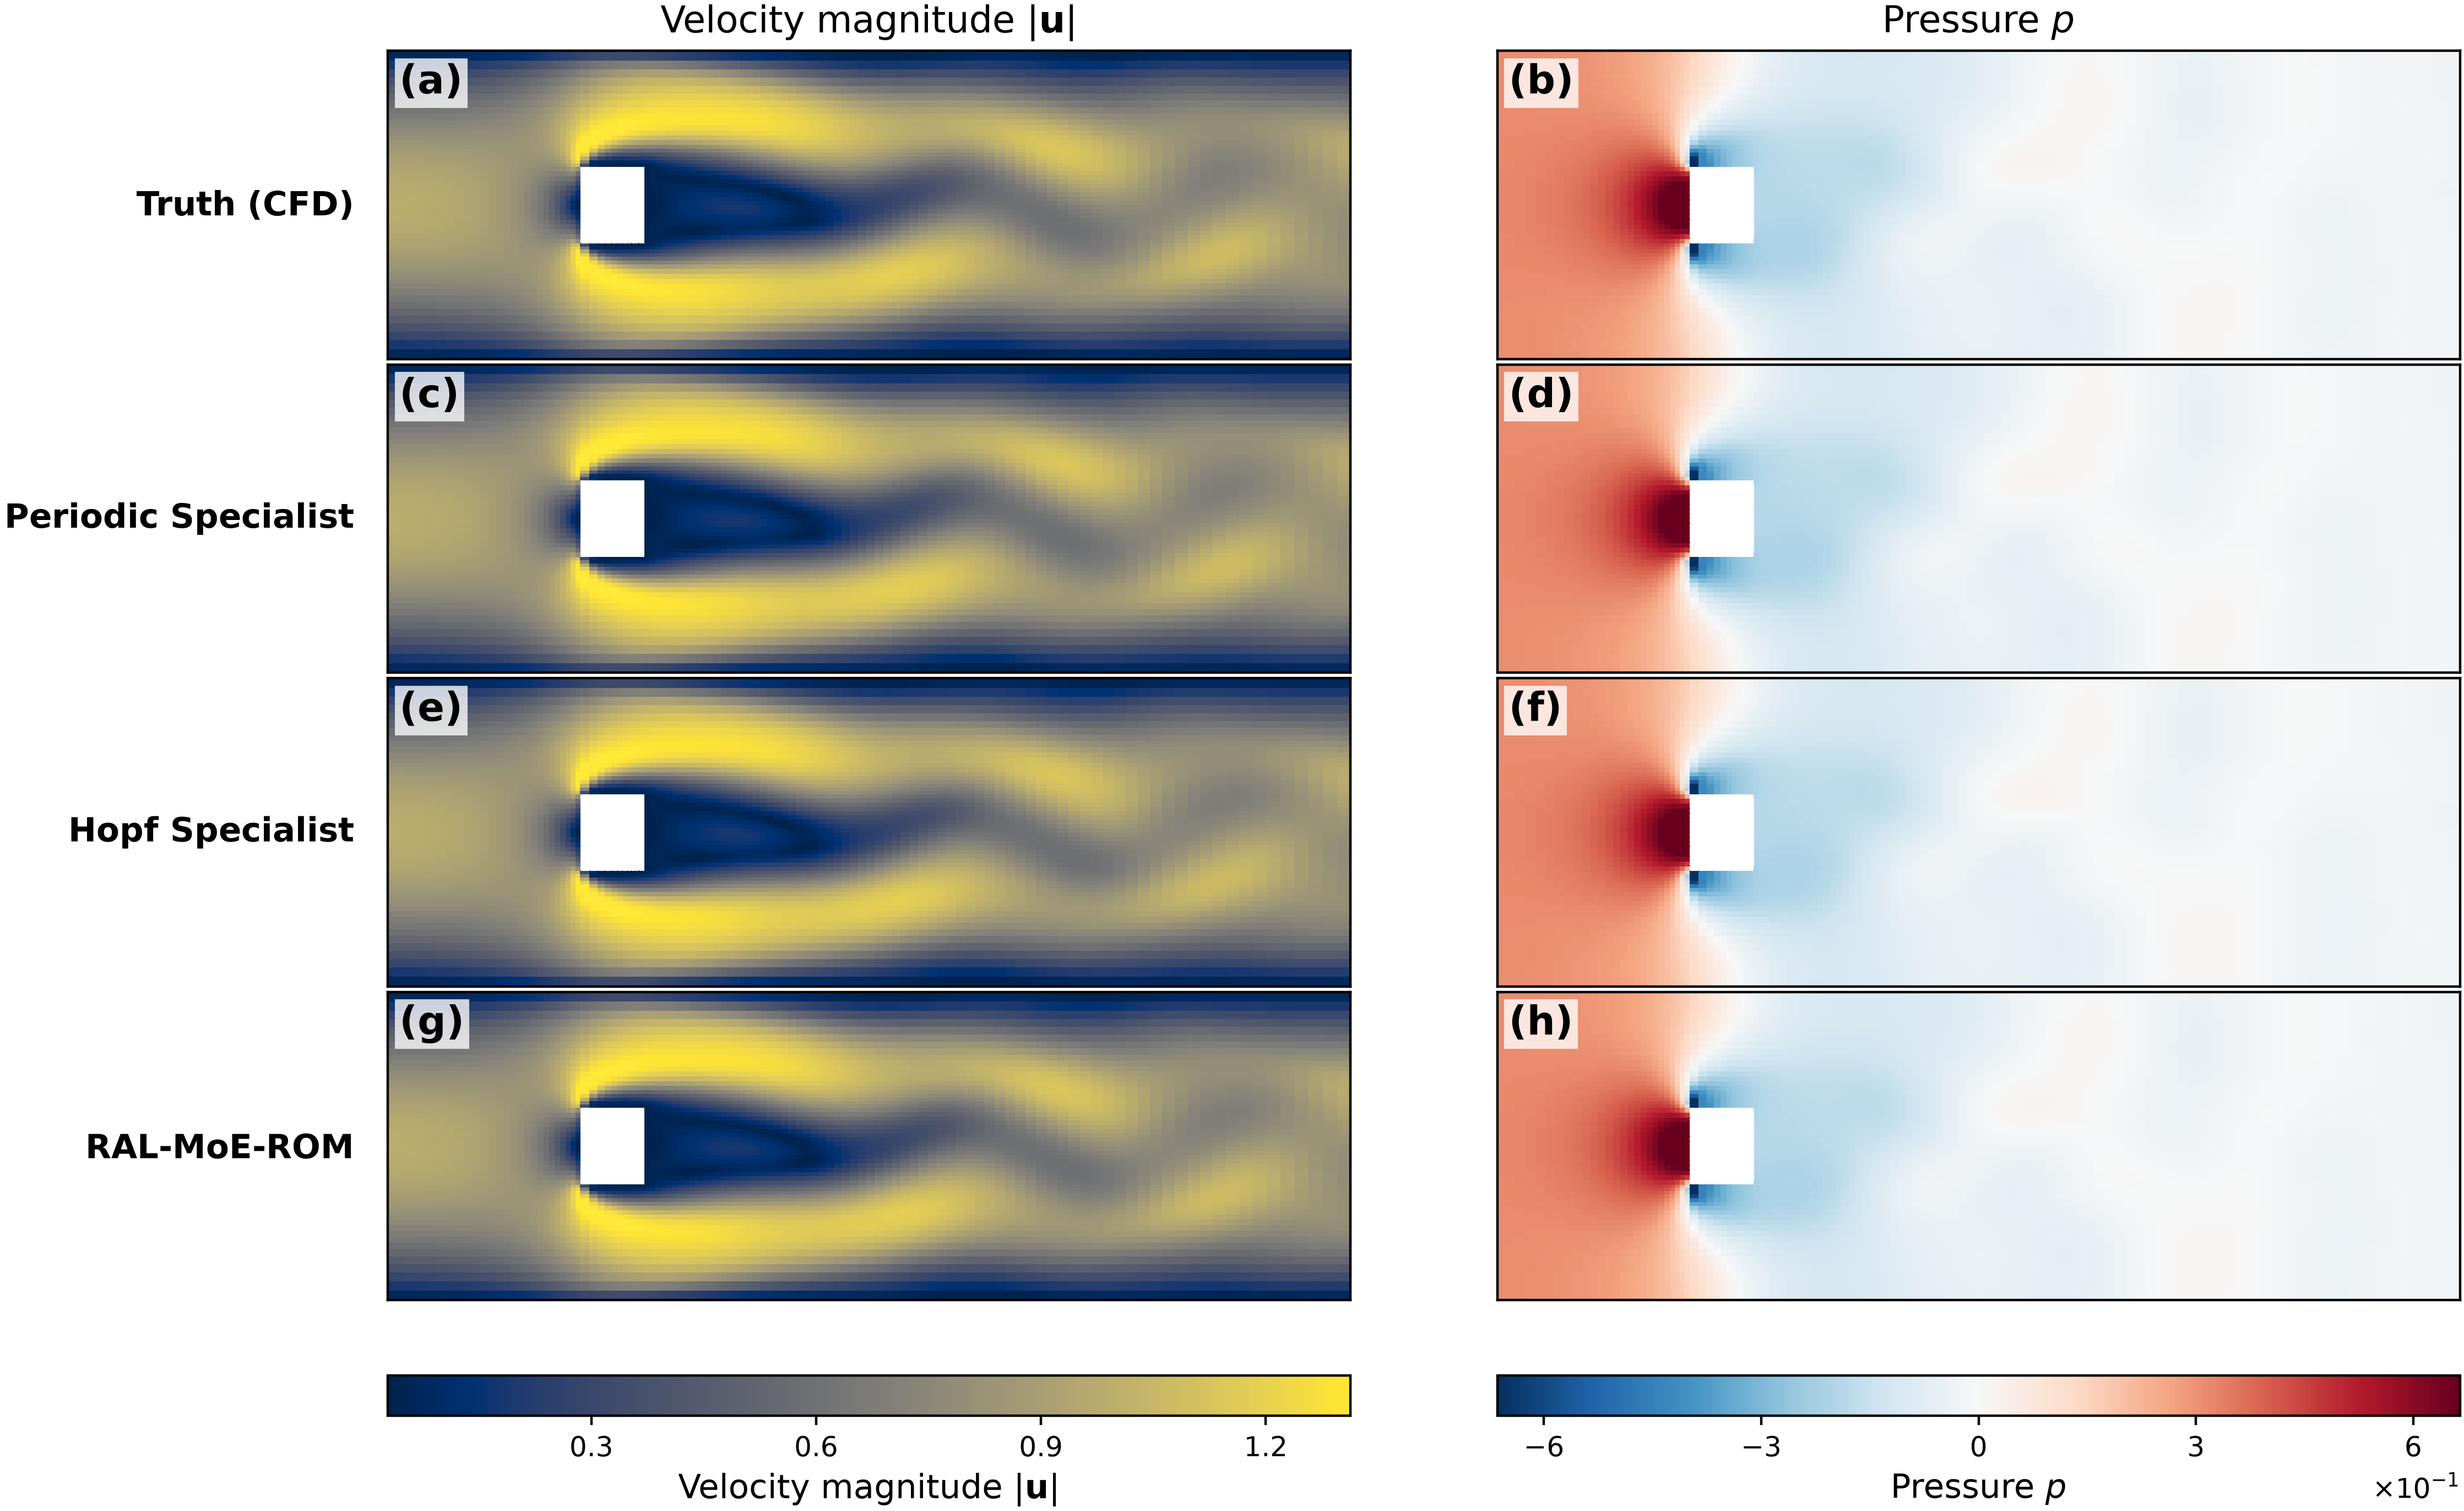
\includegraphics[width=0.95\linewidth]{figures/verified_20260920/HP_fields.png}

\vspace{0.35em}
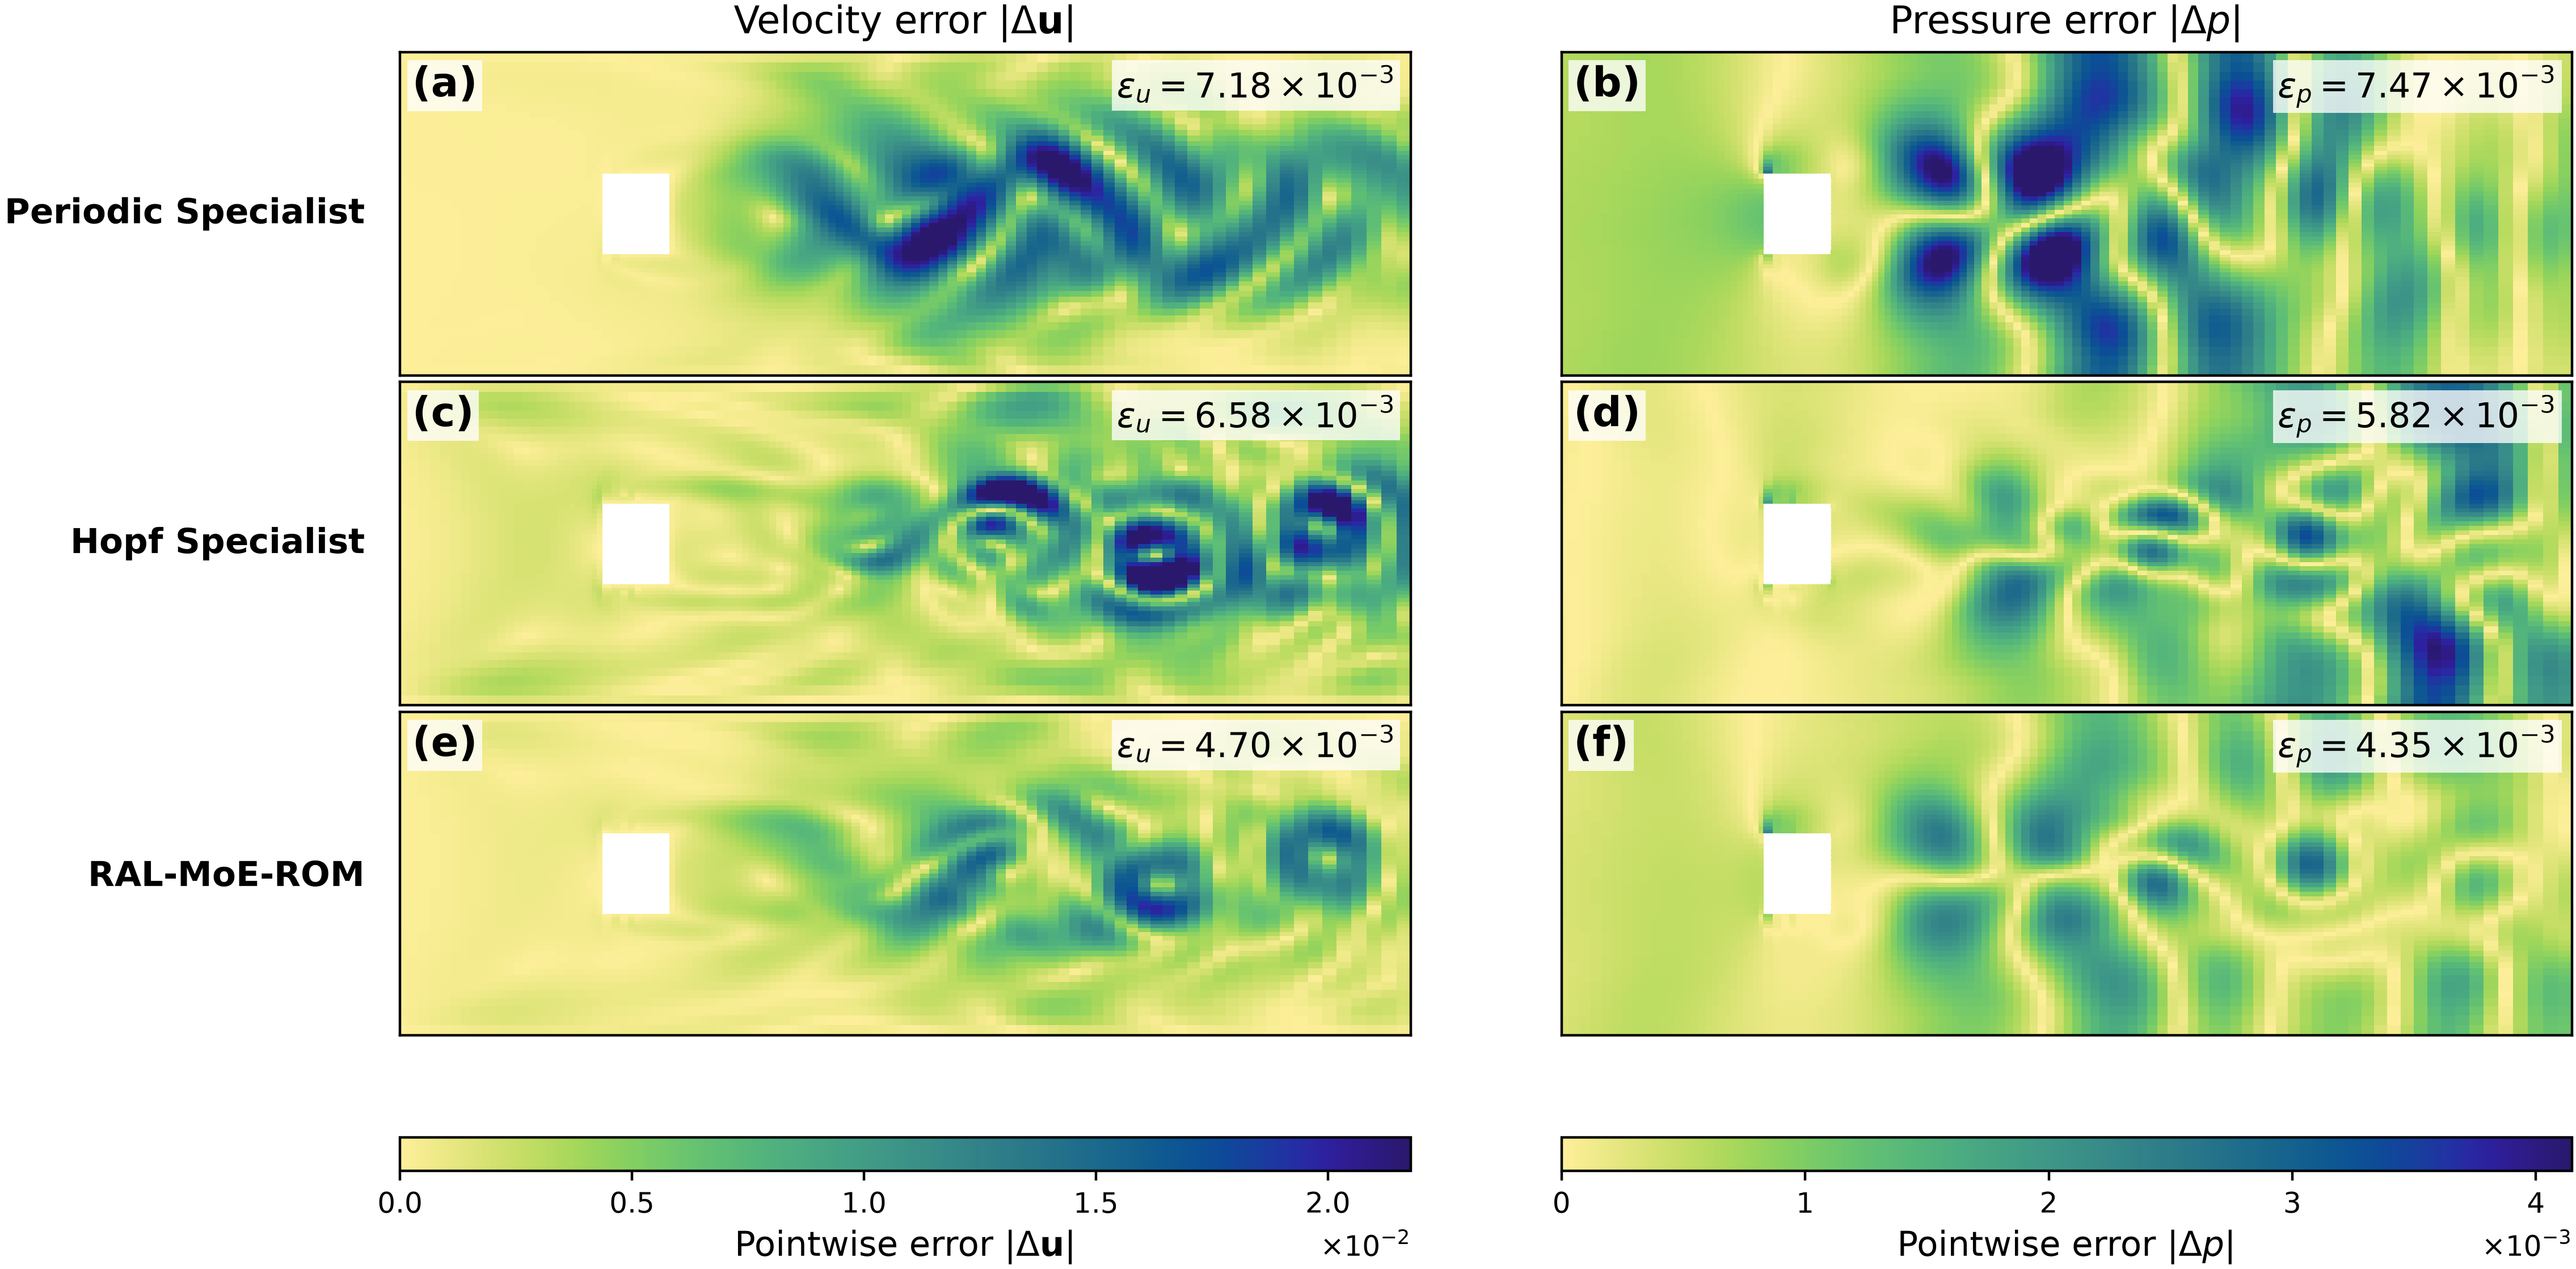
\includegraphics[width=0.95\linewidth]{figures/verified_20260920/HP_errors.png}
\caption{Selected held-out prediction in the centered-square
$H$--$P$ overlap at $Re=100.5$, window 5, zero-based rollout index 23, $t=384$ (the $K=24$ endpoint). The upper panel compares the CFD reference, Periodic specialist, Hopf specialist, and T2-C prediction for velocity magnitude and gauge-corrected pressure. The lower panel gives velocity-vector and absolute pressure errors. Selection, shared robust scale limits (including possible saturation), and fractional relative-error annotations follow Figure~\ref{fig:app_square_sh_full}. This selected snapshot does not replace aggregate evaluation.}
\label{fig:app_square_hp_full}
\end{figure}
\par
